%!TEX root=./LIVRO.tex
\chapter{O que dizem os números}
\markboth{Módulo 1}{}

\vspace*{-1cm}

\section{Habilidades do SAEB}

\begin{itemize}
  \item Escrever números racionais (naturais de até 6 ordens, representação
fracionária ou decimal finita até a ordem dos milésimos) em sua
representação por algarismos ou em língua materna ou associar o registro
numérico ao registro em língua materna.

  \item Identificar a ordem ocupada por um algarismo ou seu valor posicional
(ou valor relativo) em um número natural de até 6 ordens.

  \item Comparar ou ordenar números racionais (naturais de até 6 ordens,
representação fracionária ou decimal finita até a ordem dos milésimos),
com ou sem suporte da reta numérica.

  \item Compor ou decompor números naturais de até 6 ordens na forma aditiva,
ou em suas ordens, ou em adições e multiplicações.

  \item Comparar diferentes sentenças de adições ou de subtrações de dois
números naturais.

  \item Determinar o número desconhecido que torna verdadeira uma igualdade
que envolve as operações fundamentais com números naturais de até 6
ordens.
\end{itemize}

\subsection{Habilidades da BNCC}

\begin{itemize}
\item EF03MA01, EF03MA04.
\end{itemize}

\conteudo{Neste módulo, é necessário revisar os conceitos de montagem 
de números, frisando muito as classes e até a 6º ordem. É muito importante
os alunos saírem deste módulo sabendo o valor posicional e relativo de
cada algarismo quando estão em determinada ordem. Além disso, também
é necessário trabalhar a decomposição dos números e sua escrita por extenso.}

\conteudo{
\noindent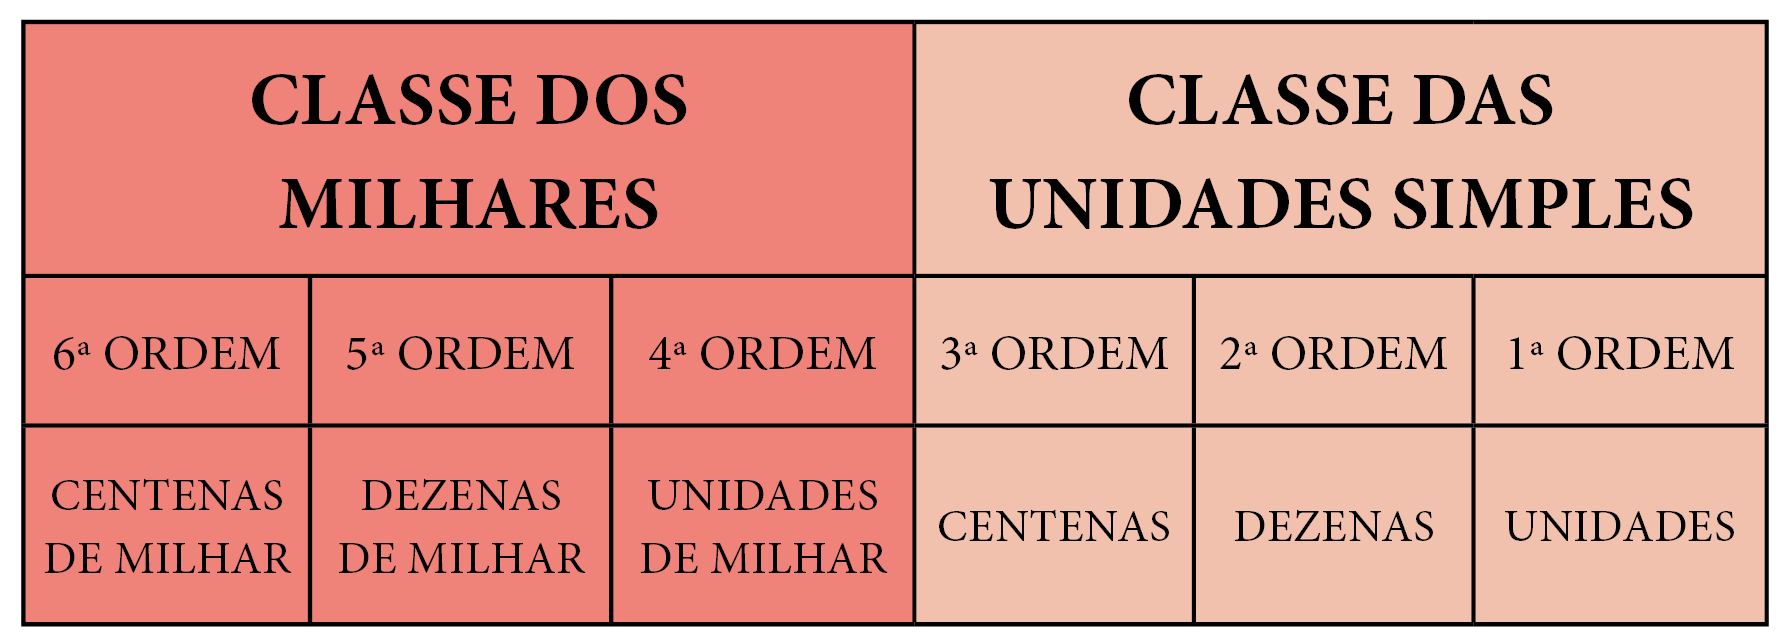
\includegraphics[width=\textwidth]{./media/image1.png}

Valor posicional ou relativo: é o valor que o algarismo assume
dependendo da classe e da ordem em que ele está posicionado no número.

Exemplo: No número 352.146, o algarismo 5 possui valor posicional ou
relativo igual a 50.000, pois ocupa a 5º ordem, a qual está dentro da
classe dos milhares; ou seja, está na posição da dezena de milhar. Sendo
assim, 5 x 10.000 = 50.000.

Decomposição numérica de acordo com a posição do algarismo:

Exemplo: 389 = 3 x 100 + 8 x 10 + 9}

\section{Atividades}

\num{1} Vilma encontrou um pedaço de papel em sua bolsa com um número escrito:

\begin{figure}[htpb!]
\centering
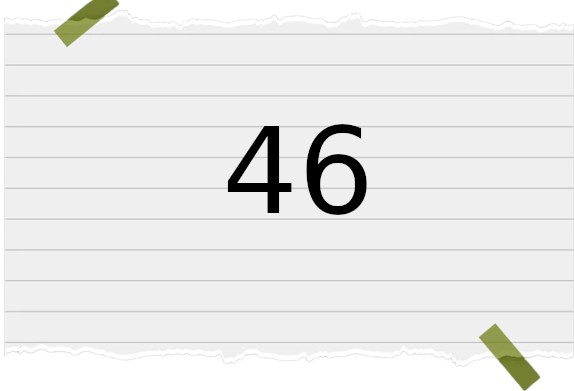
\includegraphics[width=.5\textwidth]{./media/image2.png}
\end{figure}


\begin{escolha}
\item
  Escreva por extenso como se lê esse número.
\reduline{Quarenta e seis\hfill}

\item
  Se for necessário dividir esse número em grupos de 10, quantos grupos conseguiríamos formar?
\reduline{Conseguiríamos dividir em 4 grupos com 10 unidades e sobrariam 6 unidades. 4 x 10 + 6.\hfill}
\end{escolha}

\num{2} Arnaldo estava contando suas figurinhas e, para isso, montou 8 grupos com
10 figurinhas mais 4 figurinhas em cada um deles.

\begin{escolha}
\item
  Quantas figurinhas Arnaldo possui?
\reduline{8 x 10 + 4 = 84.\hfill}
\linhas{3}

\item
  Como se escreve a quantidade de figurinhas que ele tem por extenso?
\reduline{Oitenta e quatro.\hfill}
\end{escolha}

\num{3} Treine sua criatividade escrevendo:

\begin{escolha}
\item Um número formado por três algarismos iguais.
\reduline{Resposta pessoal. Exemplo: 222.\hfill}

\item Um número formado por três algarismos no qual o 0 (zero) seja o terceiro algarismo.
\reduline{Resposta pessoal. Exemplo: 390.\hfill}

\item Um número formado por três algarismos diferentes.
\reduline{Resposta pessoal. Exemplo: 159.\hfill}

\item Um número com mais de três algarismos.
\reduline{Resposta pessoal. Exemplo: 1.477.\hfill}

\item Mostre os números que você criou para um colega e veja os que ele criou também.
\end{escolha}

\num{4} Escreva os números escritos em cada item e, depois, decomponha esse número conforme o exemplo.

\begin{myquote}\Large
\textbf{Cento e vinte e sete.}

\textbf{127 = 100 + 20 + 7}
\end{myquote}


\begin{escolha}
\item Trezentos e cinquenta e quatro.
\reduline{300 + 50 + 4\hfill}

\item Duzentos e vinte e oito.
\reduline{200 + 20 + 8\hfill}

\item Quatrocentos e setenta e seis.
\reduline{400 + 70 + 6\hfill}
\end{escolha}

\pagebreak
\num{5} Complete a tabela seguindo as instruções.\bigskip

\noindent\begin{tabular}{lll}
\hline
\begin{tabular}[c]{@{}l@{}}Número escrito\\ por extenso\end{tabular} & \begin{tabular}[c]{@{}l@{}}Número escrito\\ com algarismos\end{tabular} & Número decomposto \\ \hline
Quinhentos e vinte e seis & \rosa{526} & \rosa{500} + 20 + 6 \\
\rosa{Quatrocentos e trinta e cinco} & 435 & \rosa{400} + 30 + 5 \\
\rosa{Oitocentos e trinta e dois} & \rosa{832} & 800 + 30 + 2 \\
\rosa{Setecentos e vinte e nove} & \rosa{729} & 700 + 20 + 9 \\ \hline
\end{tabular}

\num{6} Gabriel, durante sua aula, estava aprendendo a montar números utilizando o
material dourado e montou o seguinte número:

%Produzir uma imagem semelhante a essa abaixo com 5 barras de 10 cubinhos cada e 9 cubinhos separados. Deixar a figura melhor apresentável e, se possível, numa cor parecida com o dourado.

\begin{figure}[htpb!]
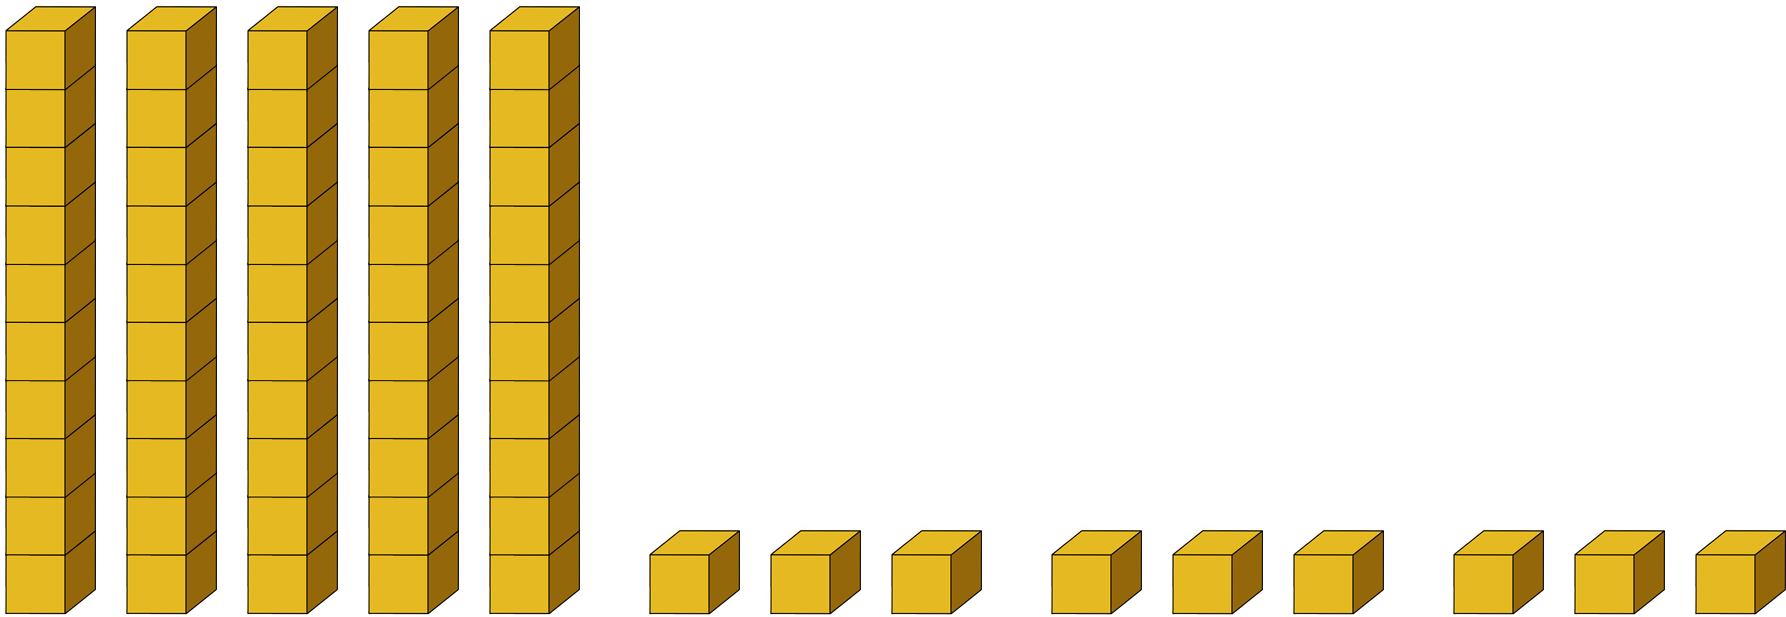
\includegraphics[width=\textwidth]{./media/image3.png}
\end{figure}

Qual é o número representado pelo material dourado na figura?
\reduline{Temos 6 dezenas e 9 unidades, portanto: 6 x 10 + 9 = 69\hfill}
\linhas{1}

\num{7} Complete os quadros abaixo com os número que indicam as quantidades e, em
seguida, escreva por extenso o número encontrado.

\begin{escolha}

\item
  Fernando tem 4 dezenas de lápis mais 2 unidades.

\begin{longtable}[]{@{}ll@{}}
\toprule
Dezena & Unidade\tabularnewline
\midrule
\endhead
&\tabularnewline
\bottomrule
\end{longtable}

Total de lápis que Fernando possui:
\reduline{4 x 10 + 2 = 42. Quarenta e dois lápis.\hfill}

\item Thiago tem 8 dezenas de bolinhas de gude mais 5 unidades.

\begin{longtable}[]{@{}ll@{}}
\toprule
Dezena & Unidade\tabularnewline
\midrule
\endhead
&\tabularnewline
\bottomrule
\end{longtable}

Total de bolinhas de gude que Thiago possui:
\reduline{8 x 10 + 5 = 85. Oitenta e cinco bolinhas de gude.\hfill}
\end{escolha}

\num{8} Realize a decomposição dos números indicados em cada item.

\begin{escolha}
\item 56: \reduline{5 x 10 + 6 = 56\hfill}

\item 73: \reduline{7 x 10 + 3 = 73\hfill}

\item 94: \reduline{9 x 10 + 4 = 94\hfill}

\item 14: \reduline{1 x 10 + 4 = 14\hfill}

\item 81: \reduline{8 x 10 + 1 = 81\hfill}

\item 158: \reduline{1 x 100 + 5 x 10 + 8 = 158\hfill}

\item 649: \reduline{6 x 100 + 4 x 10 + 9\hfill}

\item 784: \reduline{7 x 100 + 8 x 10 + 4\hfill}
\end{escolha}

\pagebreak
\num{9} Richard encontrou as seguintes peças de um material dourado:

\begin{figure}[htpb!]
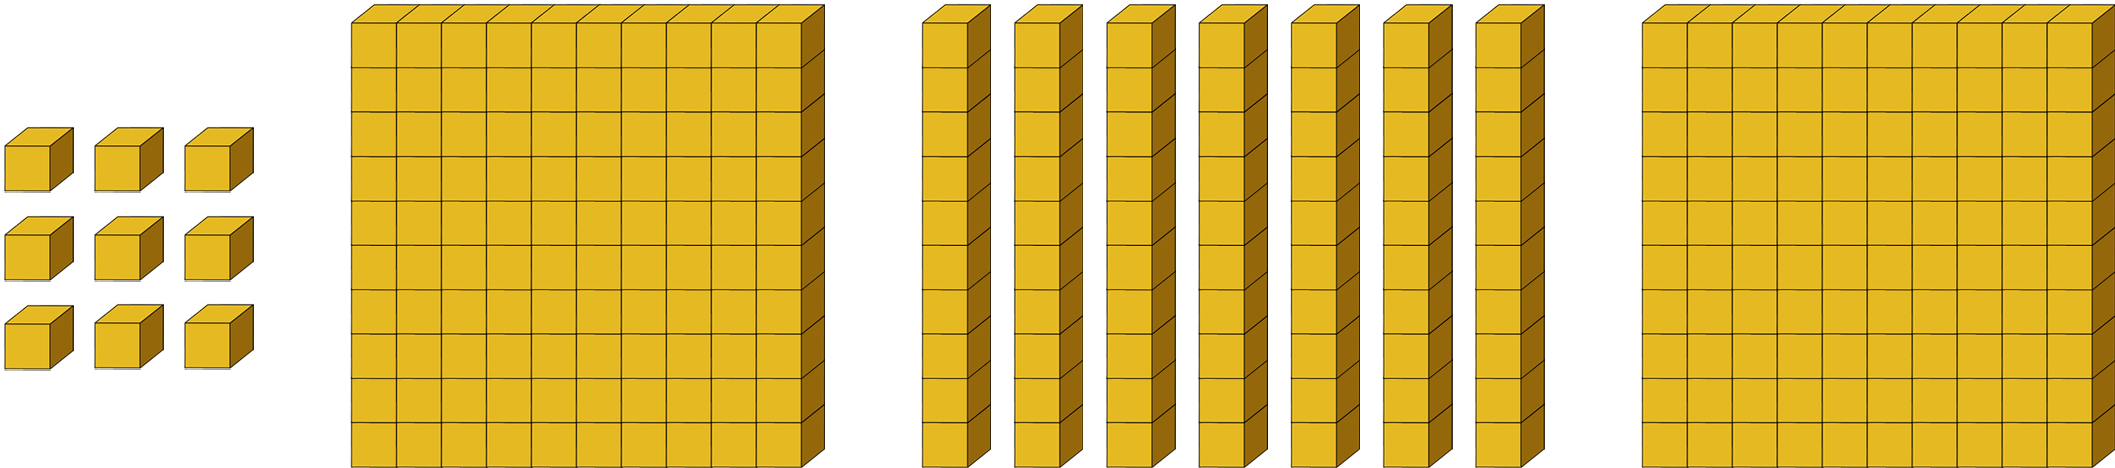
\includegraphics[width=\textwidth]{./media/image4.png}
\end{figure}

Utilizando todas as peças, qual o maior número que Richard conseguirá
representar? Após encontrar o número, escreva-o por extenso.
\reduline{2 x 100 + 7 x 10 + 9 = 279 (Duzentos e setenta e nove)\hfill}
\linhas{3}

\num{10} Monte os números compostos e registre-os nos locais correspondentes.

\begin{escolha}
\item 5 centenas e 4 unidades:
\reduline{504\hfill}

\item 7 dezenas e 2 unidades:
\reduline{72\hfill}

\item 9 centenas, 5 dezenas e 6 unidades:
\reduline{956\hfill}

\item 2 centenas, 6 dezenas e 3 unidades:
\reduline{263\hfill}

\end{escolha}

\pagebreak
\num{11} Ligue os retângulos da coluna 1 a um corresponde da coluna 2 que
represente a escrita por extenso do número indicado na primeira coluna.

\begin{figure}[htpb!]
\centering
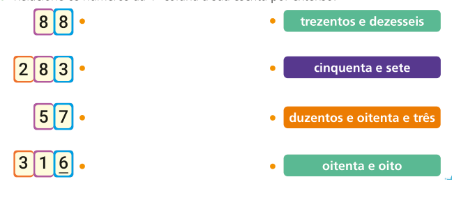
\includegraphics[width=\textwidth]{./media/image5.png}
\end{figure}

%Produzir uma figura conforme a indicada acima: (não colocar os pontos em vermelho que aparecem na figura acima). Não precisa ser colorido. Pose ser feito no padrão e cores do projeto.

%\coment{88 deve estar ligado ao oitenta e oito.
%283 deve estar ligado ao duzentos e oitenta e três.
%57 deve estar ligado a ciquenta e sete.
%316 deve estar ligado ao trezentos e dezesseis.}

\num{12} Felipe quer realizar uma corrida e resolveu planejá-la. Para isso, fez
uma linha reta e nela marcou intervalos de 1 km, conforme representado na imagem.

\begin{figure}[htpb!]
\centering
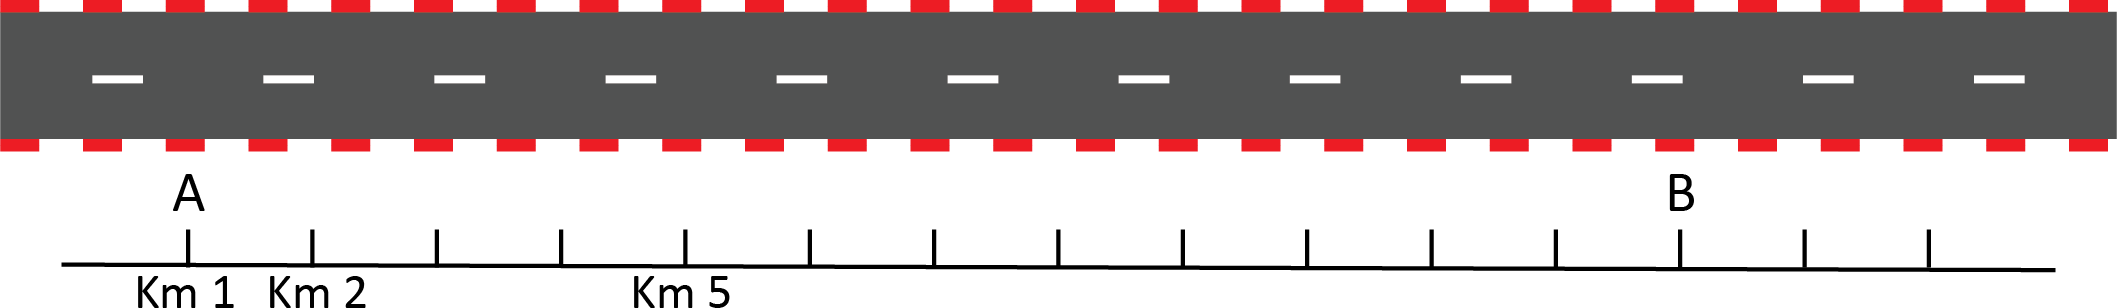
\includegraphics[width=\textwidth]{./media/image6.png}
\end{figure}


Ele pretende começar no ponto A e terminar no ponto B. Se Felipe
conseguiu completar a corrida, ele parou na marcação

\begin{minipage}{.5\textwidth}
\begin{escolha}
\item Km 9.

\item Km 10.

\item Km 11.

\item Km 12.
\end{escolha}
\end{minipage}
\sidetext{Como ele saiu do ponto A, que está em cima da marcação km 0, e chegou ao
ponto B, que está a 12 marcações de distância do ponto, podemos concluir
que ele parou no km 12; ou seja, percorreu 12 km.

Explore ao máximo com os alunos a colocação dos números na reta numérica,
já que é um conceito essencial em outros assuntos.}

\pagebreak
\num{13} A bolas representadas fazem parte de um jogo conhecido como
bilhar ou sinuca.

\begin{figure}[htpb!]
\centering
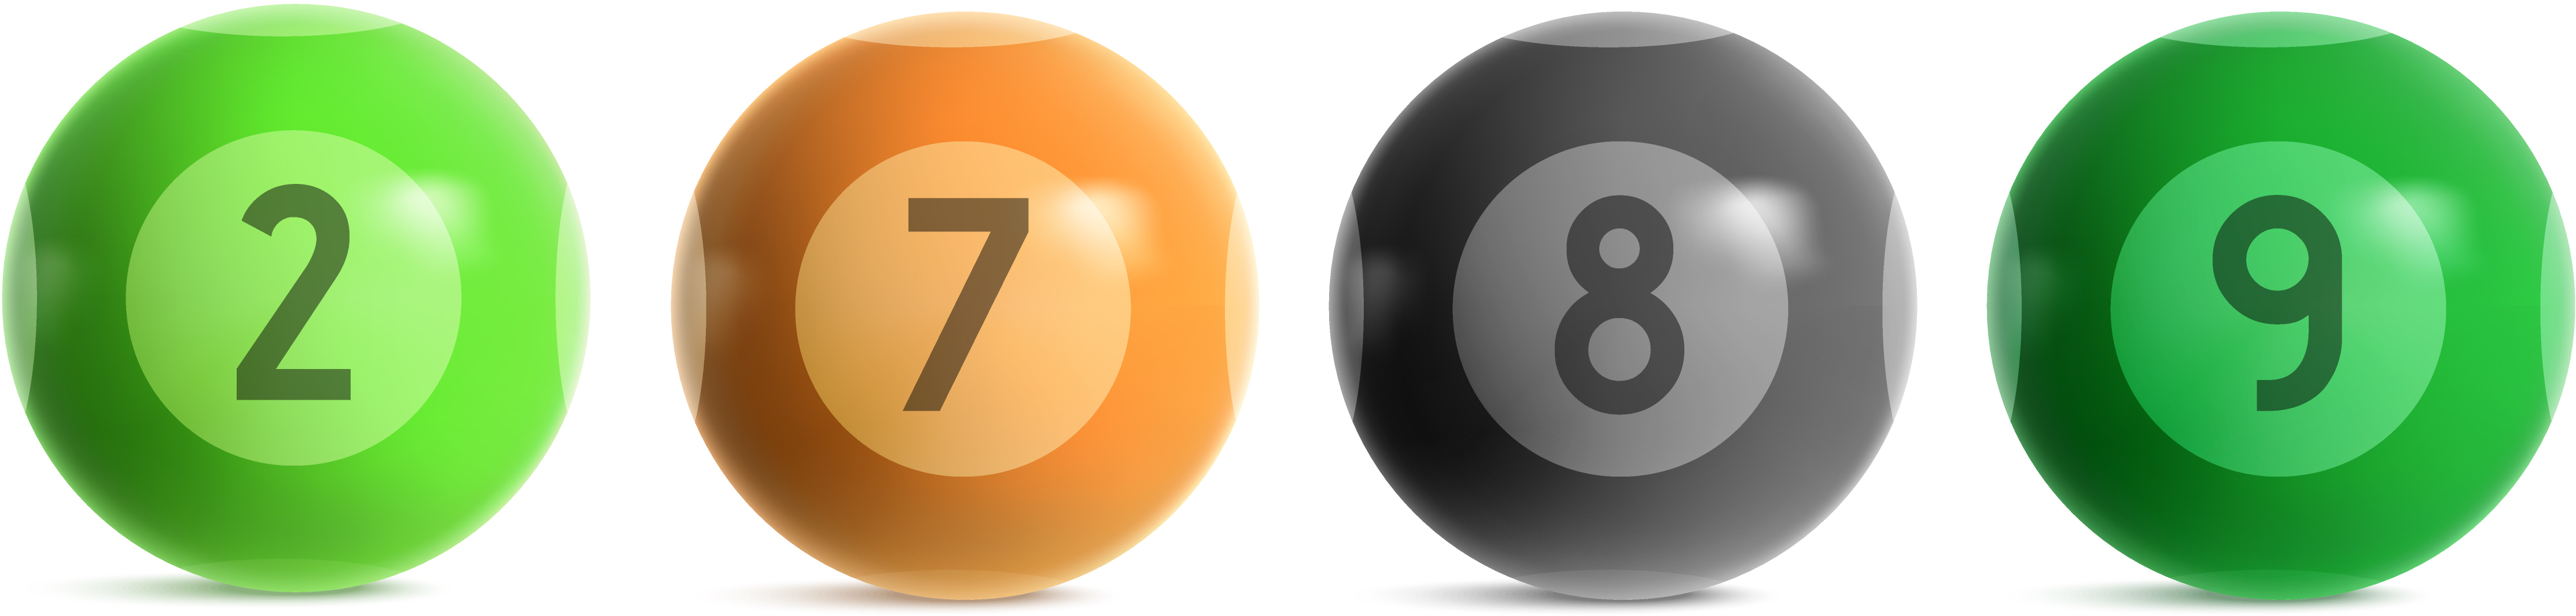
\includegraphics[width=\textwidth]{./media/image7.png}
\end{figure}

Observando os números representados em cada bola, responda:

\begin{escolha}
\item Qual o maior número?
\reduline{9 (nove)\hfill}

\item Qual o menor número com 3 exatamente ordens que podemos formar?
\reduline{278 (duzentos e setenta e oito)\hfill}

\item Qual o maior número par que podemos formar?
\reduline{9.872 (nove mil oitocentos e setenta e dois)\hfill}

\end{escolha}

\coment{Explore mais exemplos com os alunos para estimular a criatividade
e a formação de números.}

\pagebreak
\section{Treino}

\num{1} Amanda estava brincando no escritório de seu pai quando
encontrou um pedaço de papel com uma anotação.

\begin{myquote}
Faturamento diário: 734 reais
\end{myquote}

Lembrando das aulas de matemática, ela resolveu decompor o número escrito
no papel. Qual a decomposição correta que Amanda deverá fazer desse
número?

\begin{escolha}
\item
  700 + 30 + 4
\item
  70 + 3 + 4
\item
  700 + 40 + 3
\item
  70 + 300 + 4
\end{escolha}

\num{2} Na reta numérica a seguir, o ponto P representa o número 540 e o ponto U representa o número 590.

\begin{figure}[htpb!]
\centering
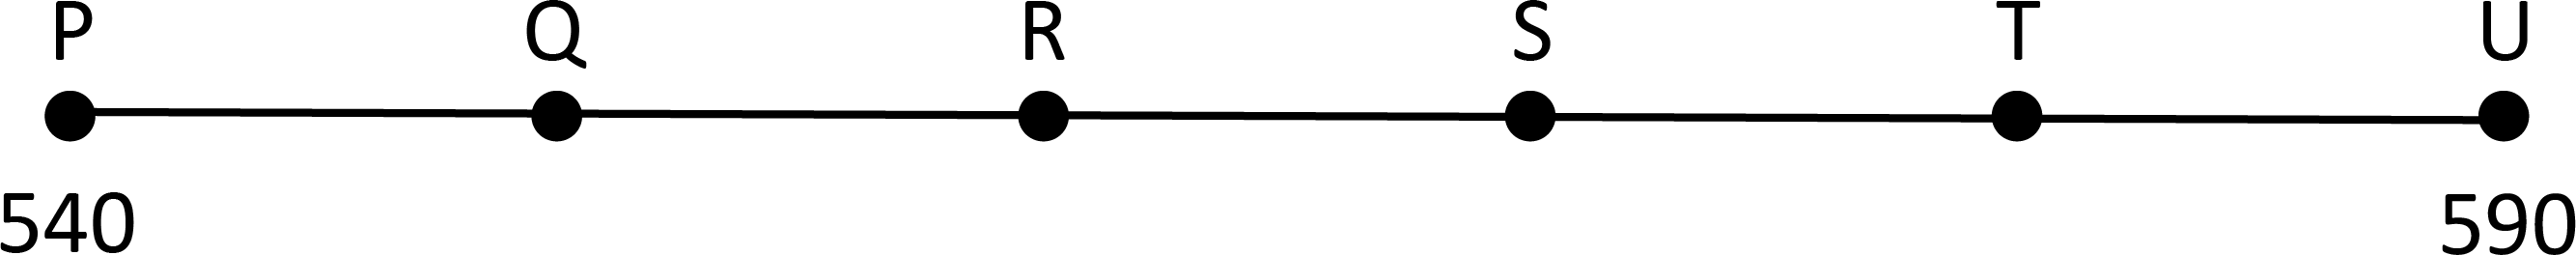
\includegraphics[width=\textwidth]{./media/image8.png}
\end{figure}

Em qual ponto temos a representação do número 570, sabendo-se que a
distância entre dois pontos consecutivos é de 10 unidades?

\begin{escolha}
\item
  Q
\item
  R
\item
  S
\item
  T
\end{escolha}

\pagebreak
\num{3} Utilizando o material dourado, Ana Letícia montou a seguinte número:

\begin{figure}[htpb!]
\centering
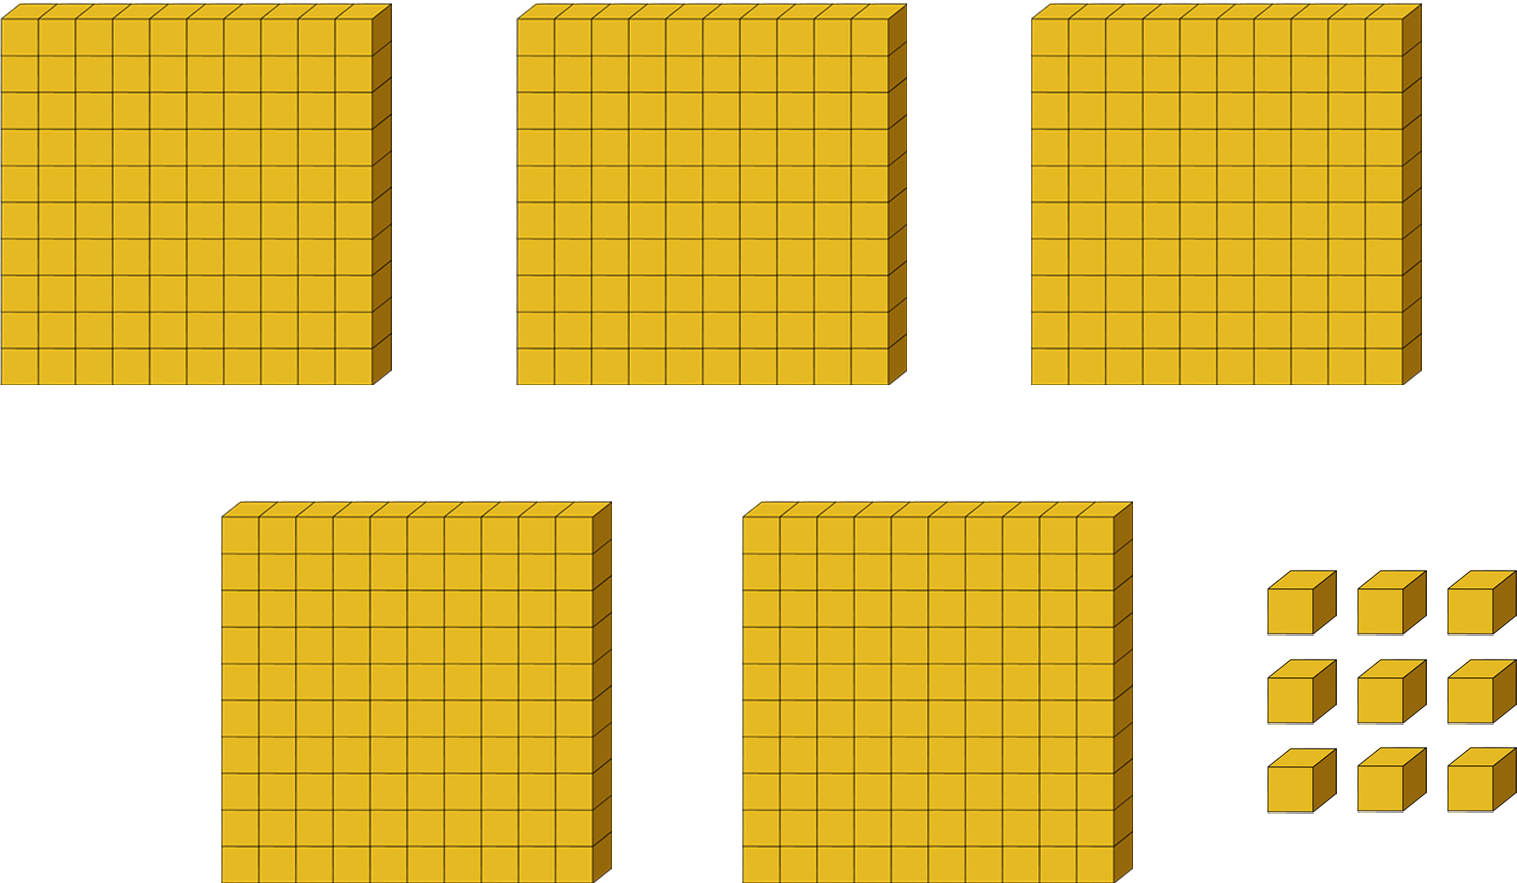
\includegraphics[width=\textwidth]{./media/image9.png}
\end{figure}

Qual o número representado por Ana Letícia?

\begin{escolha}
\item
  59
\item
  159
\item
  509
\item
  1.509
\end{escolha}


\chapter{Cálculos}
\markboth{Módulo 2}{}

\section{Habilidades do SAEB}

\begin{itemize}
\item Calcular o resultado de adições ou subtrações envolvendo números
naturais de até 6 ordens.

\item Calcular o resultado de multiplicações ou divisões envolvendo números
naturais de até 6 ordens.

\item Associar o quociente de uma divisão com resto zero de um número
natural de até 6 ordens por 2, 3, 4, 5 e 10 às ideias de metade, terça,
quarta, quinta e décima parte.

\item Resolver problemas de adição ou de subtração, envolvendo números
naturais de até 6 ordens, com os significados de juntar, acrescentar,
separar, retirar, comparar ou completar.

\item Resolver problemas de multiplicação ou de divisão, envolvendo números
naturais de até 6 ordens, com os significados de formação de grupos
iguais (incluindo repartição equitativa e medida), proporcionalidade ou
disposição retangular.
\end{itemize}

\subsection{Habilidades da BNCC}

\begin{itemize}
\item EF03MA06, EF03MA07, EF03MA08.
\end{itemize}

\conteudo{
Assim como todos os conteúdos que envolvem as quatro operações básicas, este módulo é essencial e seu estudo deve ser feito com tempo para bastante treino. Relembre com os alunos cada detalhe
e os algoritmos de adição, subtração, multiplicação e divisão, dando 
ênfase à divisão, que geralmente é o maior desafio enfrentado pelos alunos.
}

\conteudo{
\begin{itemize}
\item Adição:
\end{itemize}\bigskip

\noindent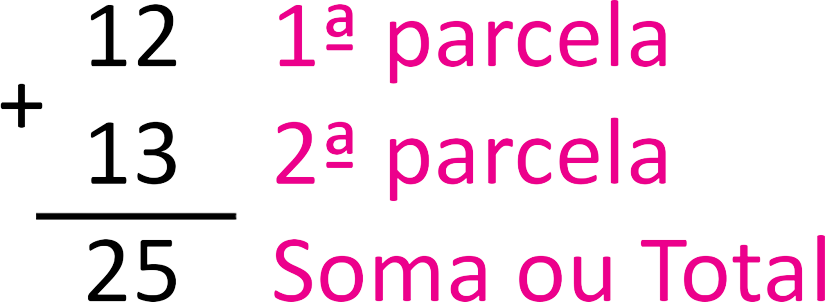
\includegraphics[width=.5\textwidth]{./media/image10.png}

\begin{itemize}
\item Subtração:
\end{itemize}

\noindent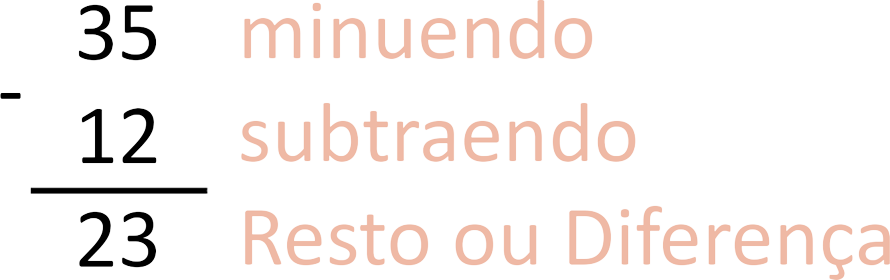
\includegraphics[width=.5\textwidth]{./media/image11.png}

\begin{itemize}
\item Multiplicação:
\end{itemize}

\noindent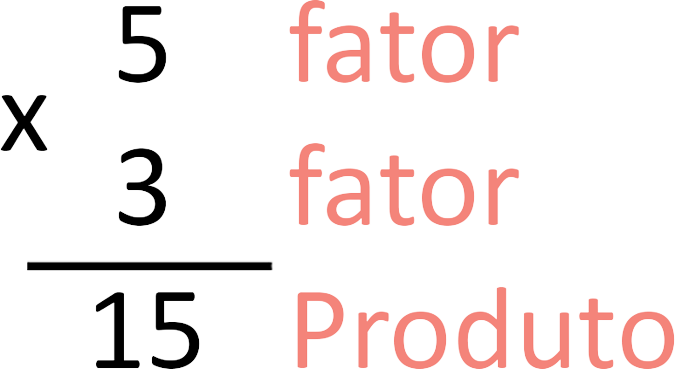
\includegraphics[width=.5\textwidth]{./media/image12.png}

\begin{itemize}
\item Divisão:
\end{itemize}

\noindent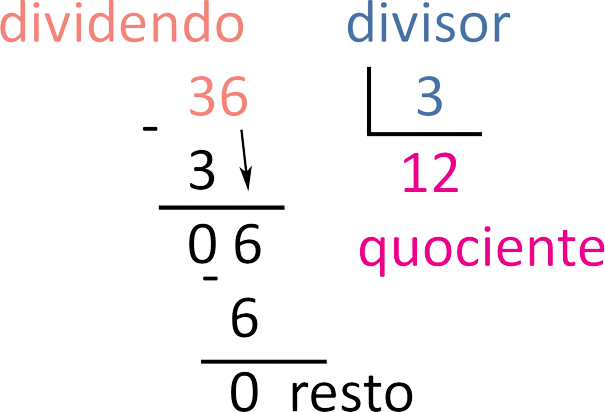
\includegraphics[width=.5\textwidth]{./media/image13.png}
}

\section{Atividades}

\num{1} Assinale o que deve ser feito em cada item para que ocorra o que se pede.

\begin{escolha}

\item
  Transformar 262 em 362.

\begin{boxlist}
\boxitem{\white{X}} Adicionar 1.

\boxitem{\white{X}} Adicionar 10.

\boxitem{\white{X}} Adicionar 100.
\end{boxlist}

\item
  Transformar 1.100 em 1.000.

\begin{boxlist}
\boxitem{\white{X}} Subtrair 1.

\boxitem{\white{X}} Subtrair 10.

\boxitem{\white{X}} Subtrair 100.
\end{boxlist}

\item
  Transformar 238 em 239.

\begin{boxlist}
\boxitem{\white{X}} Adicionar 1.

\boxitem{\white{X}} Subtrair 1.

\boxitem{\white{X}} Adicionar 10.
\end{boxlist}

\end{escolha}

\num{2} Utilize os sinais \textless{} (menor que), \textgreater{} (maior que) ou
= (igual a) em cada situação para comparar as quantidade representadas.\bigskip

\begin{minipage}{.5\textwidth}
\begin{escolha}
\item
  7 \reduline{Menor que, \textless{}} 14
\item
  21 \reduline{Maior que, \textgreater{}} 5
\item
  1 + 3 \reduline{Igual a, =} 2 + 2
  \end{escolha}
  \end{minipage}
\begin{minipage}{.5\textwidth}
  \begin{escolha}[start=4]
\item
  5 + 2 \reduline{Maior que, \textgreater{}} 7 -- 1
\item
  20 -- 1 \reduline{Igual a, =} 19
\item
  Treze \reduline{Menor que, \textless{}} quinze
\end{escolha}
\end{minipage}

\pagebreak
\num{3} Ligue cada operação que está na coluna 1 com o seu resultado correto na coluna 2.

\begin{multicols}{2}
\red{84 + 12}
\red{60 -- 23}
\red{67 -- 58}
\red{50 -- 2 x (5 + 15) + 2}
\red{2 + 8 -- 2 x (1 + 2)}

\blue{37}

\blue{9}

\blue{96}

\blue{4}

\blue{12}
\end{multicols}

%\coment{Explore ao máximo com os alunos o conceito de quais operações devem ser realizadas primeiro e, assim, ajude na fixação desse conceito.

\coment{84 + 12 = 96

60 -- 23 = 37

67 -- 58 = 9

50 -- 2 x (5 + 15) + 2 = 50 -- 40 + 2 = 12

2 + 8 -- 2 x (1 + 2) = 2 + 8 -- 6 = 4}


